Optimization problems are encountered in many domains: BigData, engineering, logistics, and business. An optimization problem may be defined by the couple $(S, f )$, where $S$ represents the set of feasible solutions, and $f : S \implies {\rm I\!R}$ the objective function to optimize. The objective function assigns to every solution
$s \in S$ of the search space a real number indicating its worth. The objective function
$f$ allows to define a total order relation between any pair of solutions in the search
space.\\

The global optimum is defined as  a solution $s^* \in S$ and it has a better objective function than all solutions of the search space, that is, $\forall  s \in  S$, $f(s^*) 	\leq f(s)$.\\

\subsection{Metaheuristics}

\subsubsection{Definition}
The $meta$ and $heuristic$ are Greek words, $meta$ it means $higher level$ and $heuristics$ means $to$ $find$, $to$ $know$ or $to$ $discover$. Metaheuristics are a set of intelligent strategies to enhance the efficiency of heuristic procedures.\\

A metaheuristic will be successful on a given optimizaction problem if it can provide a balance between exploration and exploitation. Exploration means to generate diverse solutions so as to explore the search space on the global scale, while exploitation means search in a local region by exploiting the information that a current good solution is found in this region.
exploration, often by use of randomization, which enables an algorithm to have the ability to jump out of any local optimum so as to explore the search globally.

\subsubsection{Clasification}
The different metaheuristic approaches can be characterized by different aspects concerning the search path they follow or how memory is exploited \cite{citeulike:1859945}. A majority of these algorithms has a stochastic behavior and mimics biological or  physical processes.\\

The classification presented was proposed by Beheshti et al. \cite{Beheshti:2014:CCA:2563733.2564085}, and can be understood better as shown in the Fig.\ref{fig:classification-of-mh}.

\paragraph{Trajectory methods vs. discontinuous methods}
The different between this metaheuristics is whether they follow one single search trajectory
corresponding to a closed walk on the neighborhood graph or whether larger
jumps in the neighborhood graph are allowed. Examples of this clasificaction are: tabu search and simulated annealing. These methods usually allow moves to worse solutions to be able to escape from local minima.\\

The generation of starting solutions corresponds to jumps in the search space; these algorithms, in general, follow a discontinuous walk with respect to the neighborhood graph used in the local
search.
\paragraph{Population-based vs. single-point search}

\paragraph{Memory usage vs. memoryless methods}

\paragraph{One vs. various neighborhood structures}

\paragraph{Dynamic vs. static objective function}

\subsection{Nature-inspired vs. non-nature inspiration }

%Imagen Classification of Metaheuristic
%\squeezeup
%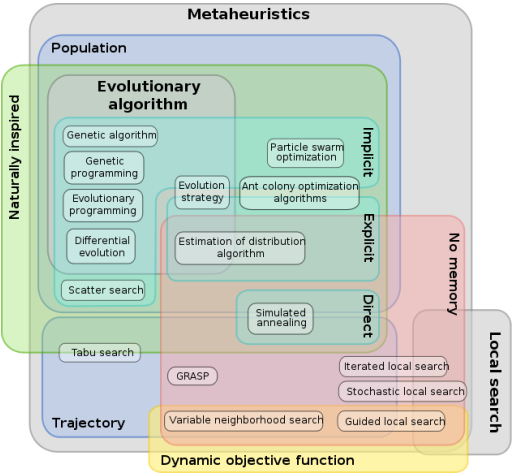
\includegraphics[]{MarcoConceptual/images/classification_mh.png} 
%\caption{Classification of Metaheuristic}\label{fig:classification-of-mh}
%\squeezeup

%TABLA (musician - > decision variables)
\squeezeup


\begin{figure}[ht]
	\centering
  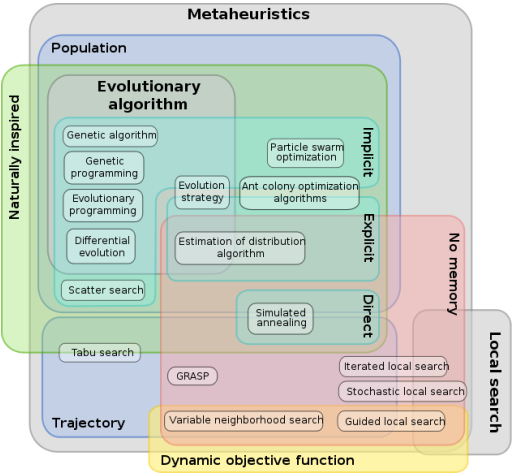
\includegraphics[width=0.55\textwidth]{MarcoConceptual/images/classification_mh.png}
	\caption{Classification of Metaheuristic}\label{fig:classification-of-mh}
\end{figure}

\squeezeup


\subsubsection{Operator} 
Unitary procedure for transforming information or implement the behavior of the algrithm.

\subsubsection{Solution} 
Array of $n$ columns containing a solution for a given problem. In the binary case, the posible values are $0$ and $1$.

\subsubsection{Constrain} 
Conditions to be met to find a viable solution.

\subsubsection{Benchmark} 
Optimal set of known problem instances to validate the propose algorithm.

\subsubsection{Objective Function}  
Implements the mathematical expression representing the problem to solve. The guiding objective function is related to the goal to achieve.

\subsubsection{Fitness} 
Value resulting by applying the objective function to solution.

\subsubsection{Matrix of Costs} 
Consist of $n$ columns vector containing the cost associated with each problem variable.

\subsubsection{Optimal Value} 
Solution with the best fitness.

\subsubsection{Domain} 
Set of possible values for the variable.

\subsubsection{Matrix A} 
Matrix containing the restrictions for the given problem.

\subsubsection{RPD} 
Relative Percentage Deviation.

\subsubsection{Harmony Memory} 
Memory space which includes the population of the solution vectors.

\subsubsection{Harmony Memory Size} 
Defines the amount of harmonies that can be stored in HM.

\subsubsection{Harmony Memory Consideration Rate (HMCR)} 
In memory consideration, the value of decision variable ${x\textprime}_1$ is randomly selected from the historical values, other decision variables, $({x\textprime}_2, {x\textprime}_3,\dots,{x\textprime}_N)$ are sequentially selected in the same manner with probability where HMCR $\in$ (0,1).

\subsubsection{Pitch Adjusting Rate (PAR)} 
Each decision variable ${x\textprime}_i$ assigned a value by memory considerations is pitch adjusted with the probability of PAR where PAR $\in$ (0,1).



